\chapter{Conception}

La conception sépare les responsabilités transactionnelles, l'expérience utilisateur et le calcul d'intelligence artificielle afin de réduire le couplage et de garder les décisions critiques vérifiables.


\section{Choix d'architecture}

Le cahier des charges initial mettait l'accent sur FastAPI. Or, le socle transactionnel du projet a été stabilisé en Spring Boot. La décision finale conserve Spring comme coeur métier et exploite FastAPI comme microservice IA. Cette adaptation respecte les capacités demandées tout en évitant une réécriture risquée.


\textbf{Décision structurante}

Spring Boot est la frontière de sécurité et la source des réponses publiques. FastAPI ne reçoit que les documents nécessaires à l'indexation et renvoie des identifiants classés. Avant affichage, Spring recharge toujours les annonces depuis MySQL.


\begin{figure}[H]
\centering
\begin{adjustbox}{max width=\textwidth,max height=.64\textheight}
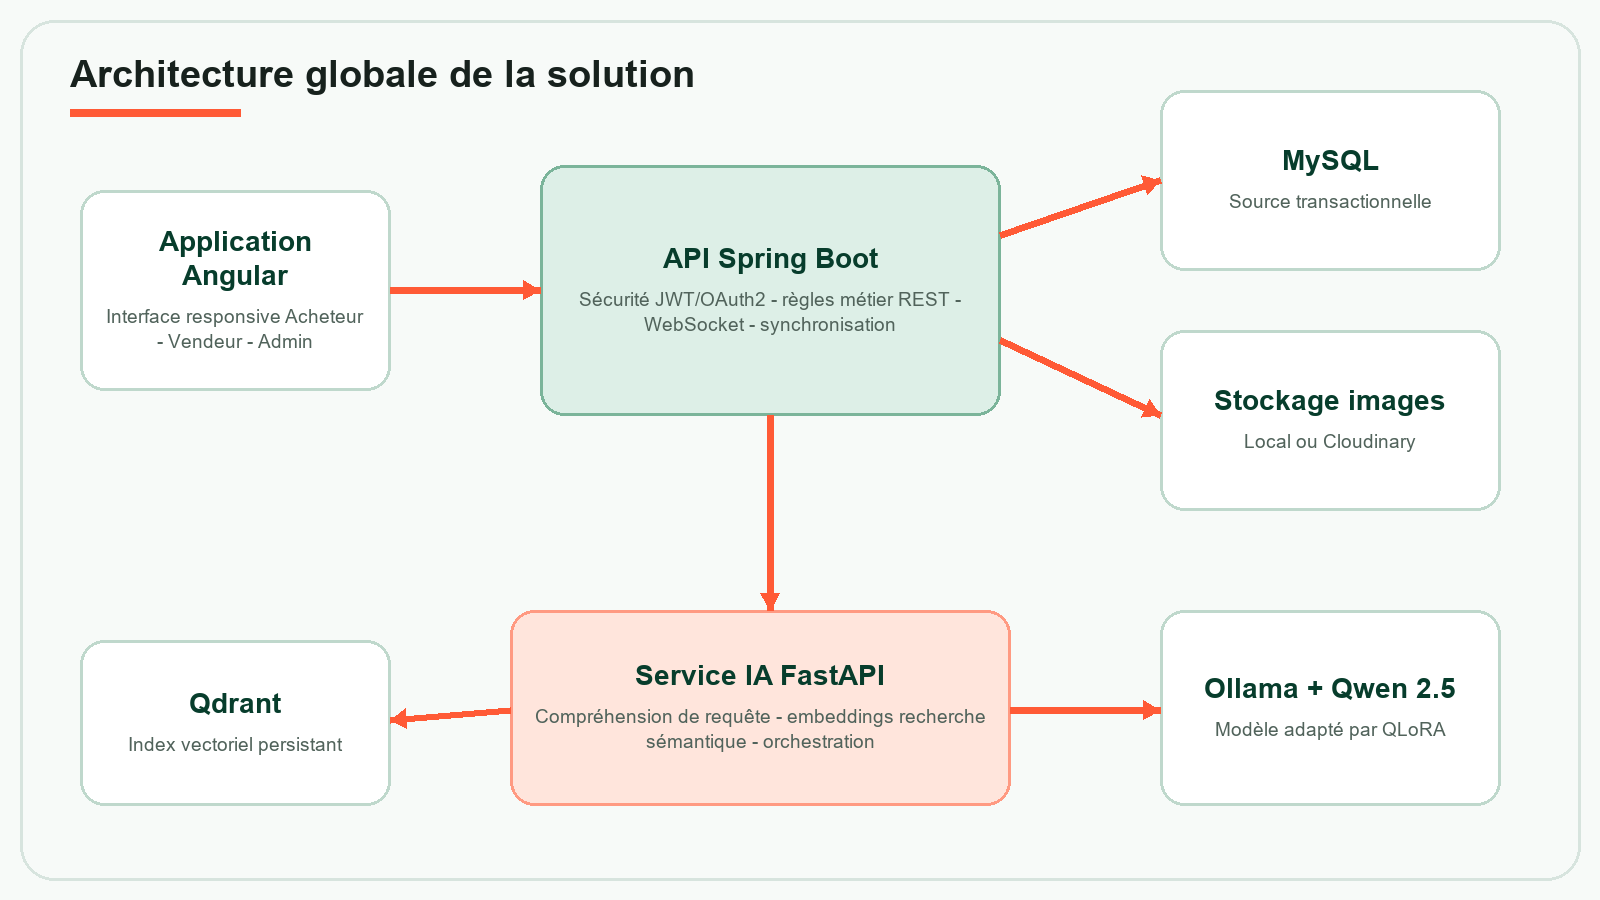
\includegraphics{images/figure-03.png}
\end{adjustbox}

\caption{Architecture globale de la solution}
\label{fig:report-3}
\end{figure}

\section{Architecture logique}

{\small\singlespacing\arrayrulecolor{tableline}
\begin{longtable}{|>{\raggedright\arraybackslash}p{\dimexpr 0.350\textwidth-2\tabcolsep-2\arrayrulewidth\relax}|>{\raggedright\arraybackslash}p{\dimexpr 0.650\textwidth-2\tabcolsep-2\arrayrulewidth\relax}|}
\hline
\rowcolor{tablehead} \color{white}\bfseries Couche & \color{white}\bfseries Responsabilité \\ \hline
\endfirsthead
\rowcolor{tablehead} \color{white}\bfseries Couche & \color{white}\bfseries Responsabilité \\ \hline
\endhead
\hline\endfoot
Présentation & Composants Angular, routes, formulaires, thèmes, retours d'erreur et accessibilité. \\ \hline
\rowcolor{tablerow} API & Contrôleurs REST, validation des DTO, sérialisation stable et contrats HTTP. \\ \hline
Métier & Services Spring portant autorisation, règles de cycle de vie, modération et classement. \\ \hline
\rowcolor{tablerow} Persistance & Dépôts JPA et modèle relationnel MySQL ; Qdrant pour les vecteurs reconstruisibles. \\ \hline
IA & Embeddings, extraction de contraintes, récupération, agents spécialisés et explications. \\ \hline
\rowcolor{tablerow} Infrastructure & Stockage d'images, courriel/SMS optionnels, OAuth et catalogue véhicule externe avec repli local. \\ \hline
\end{longtable}
}


\section{Modèle de données}

L'entité Utilisateur centralise l'identité et le rôle. Une annonce appartient à un vendeur, à une catégorie et à une collection de véhicules compatibles. Les images conservent un ordre et une image principale. Les conversations relient un acheteur, un vendeur et l'annonce d'origine. Les signaux d'activité restent séparés des messages et des coordonnées afin de limiter les données utilisées pour la personnalisation.


Les quatre vues suivantes forment le diagramme de classes du domaine persistant. Les noms correspondent aux entités Java ; les attributs sont sélectionnés pour la lisibilité. Les associations portent leurs multiplicités. Les rôles BUYER, SELLER et ADMIN sont les valeurs de UserRole, et non des sous-classes de User. Les méthodes métier appartiennent aux services, non aux entités représentées.


\clearpage

\subsection{Catalogue et favoris}

\begin{figure}[H]
\centering
\begin{adjustbox}{max width=\textwidth,max height=.64\textheight}
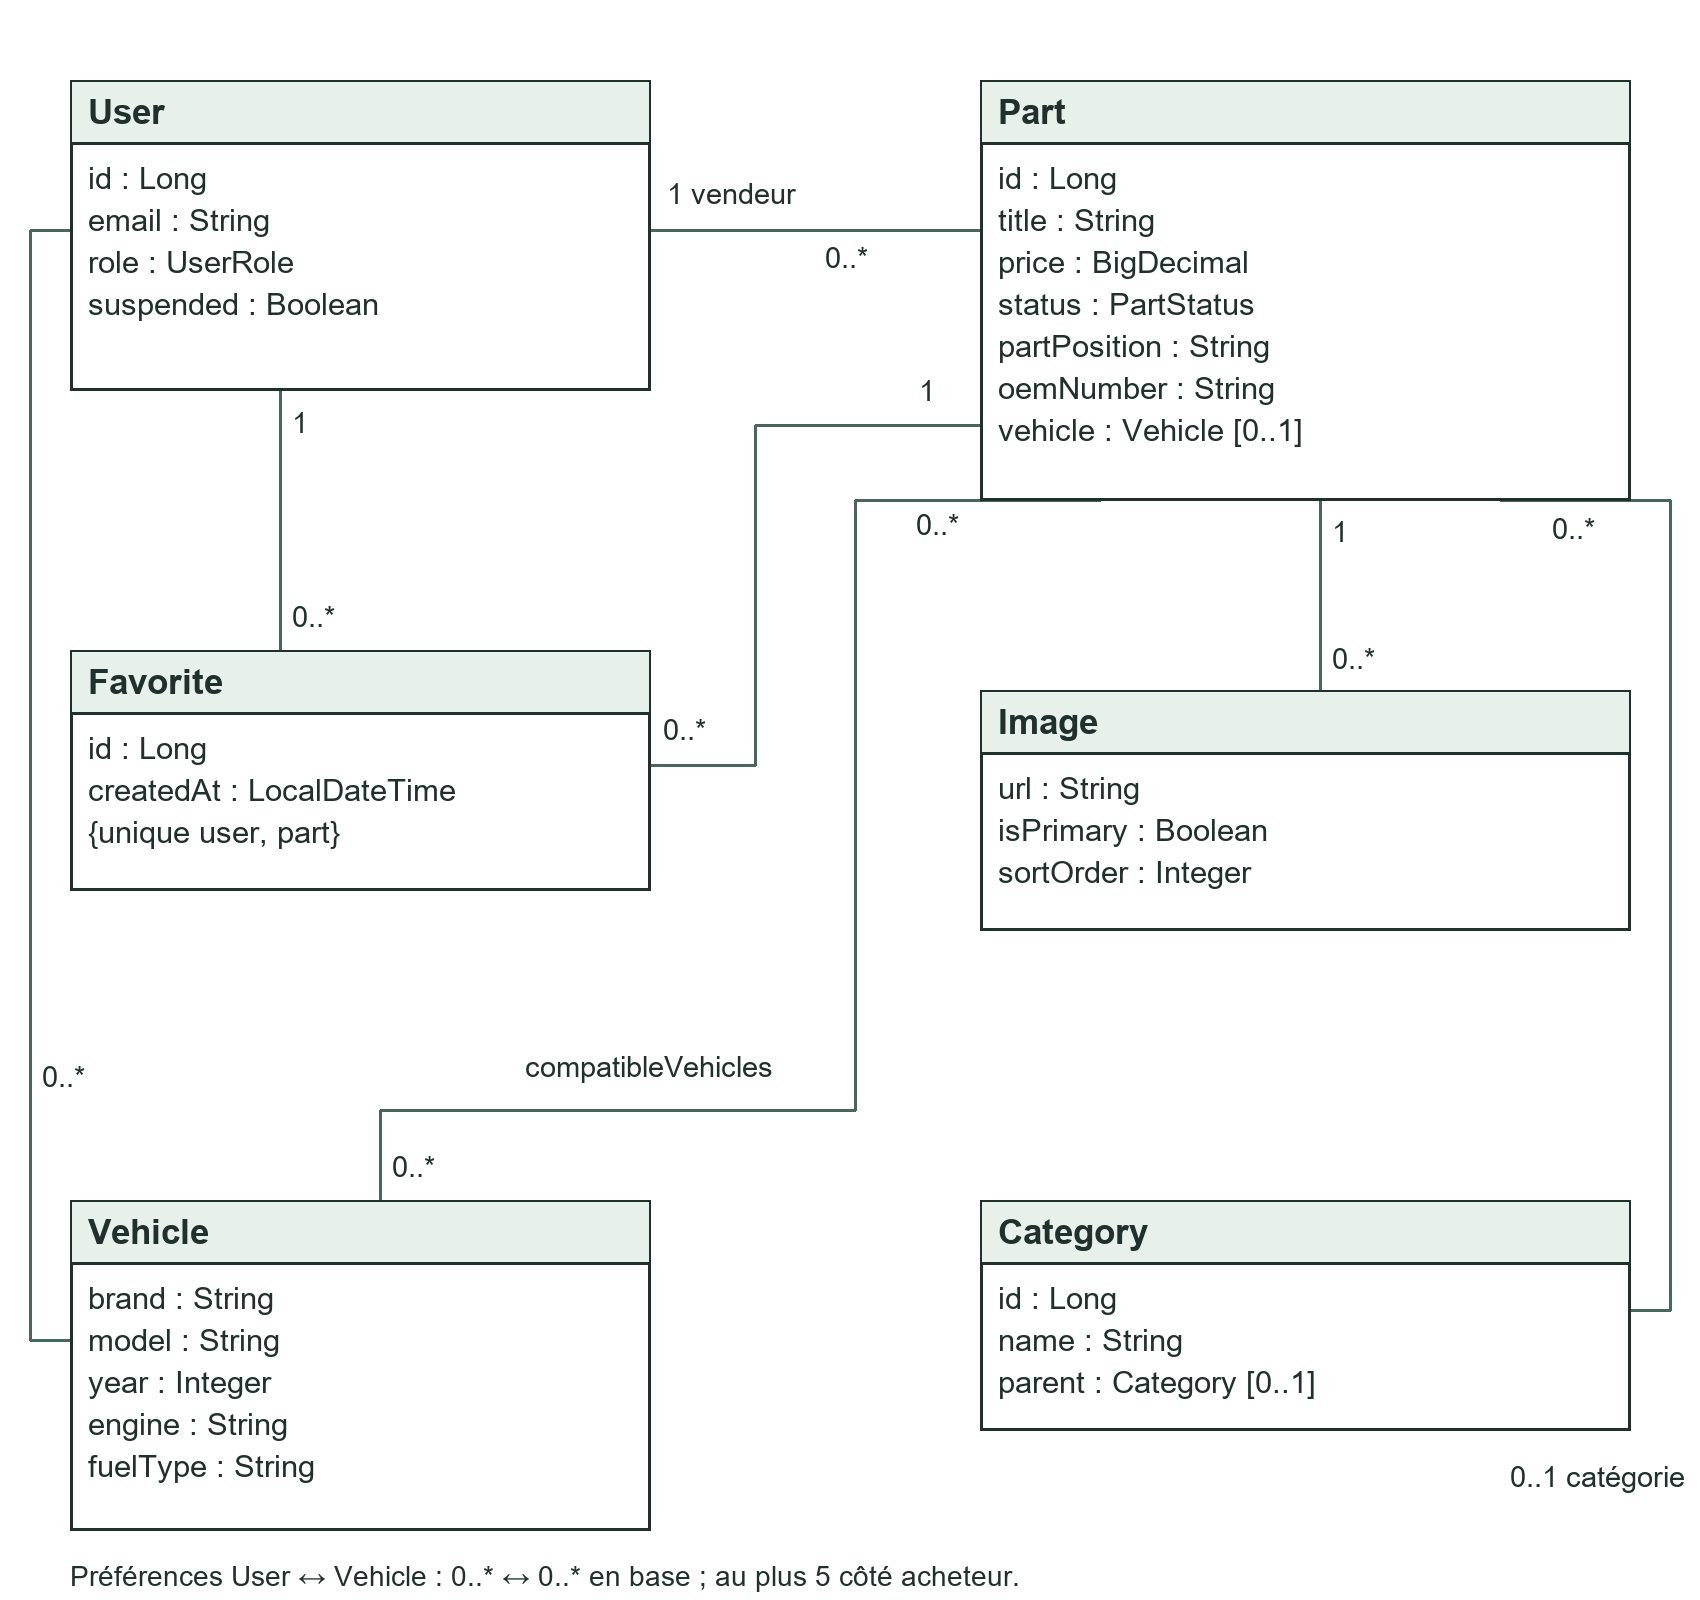
\includegraphics{images/figure-04.png}
\end{adjustbox}

\caption{Classes du catalogue et des favoris}
\label{fig:report-4}
\end{figure}

Part et Vehicle sont reliés par part\_compatible\_vehicles. Le lien historique Part.vehicle est maintenu séparément pour la compatibilité des données existantes. Category possède un parent facultatif et zéro à plusieurs sous-catégories. Les restrictions moteur et carburant de Part complètent les caractéristiques des véhicules ; elles ne constituent pas une entité de compatibilité distincte.


\clearpage

\subsection{Conversations et réputation}

\begin{figure}[H]
\centering
\begin{adjustbox}{max width=\textwidth,max height=.64\textheight}
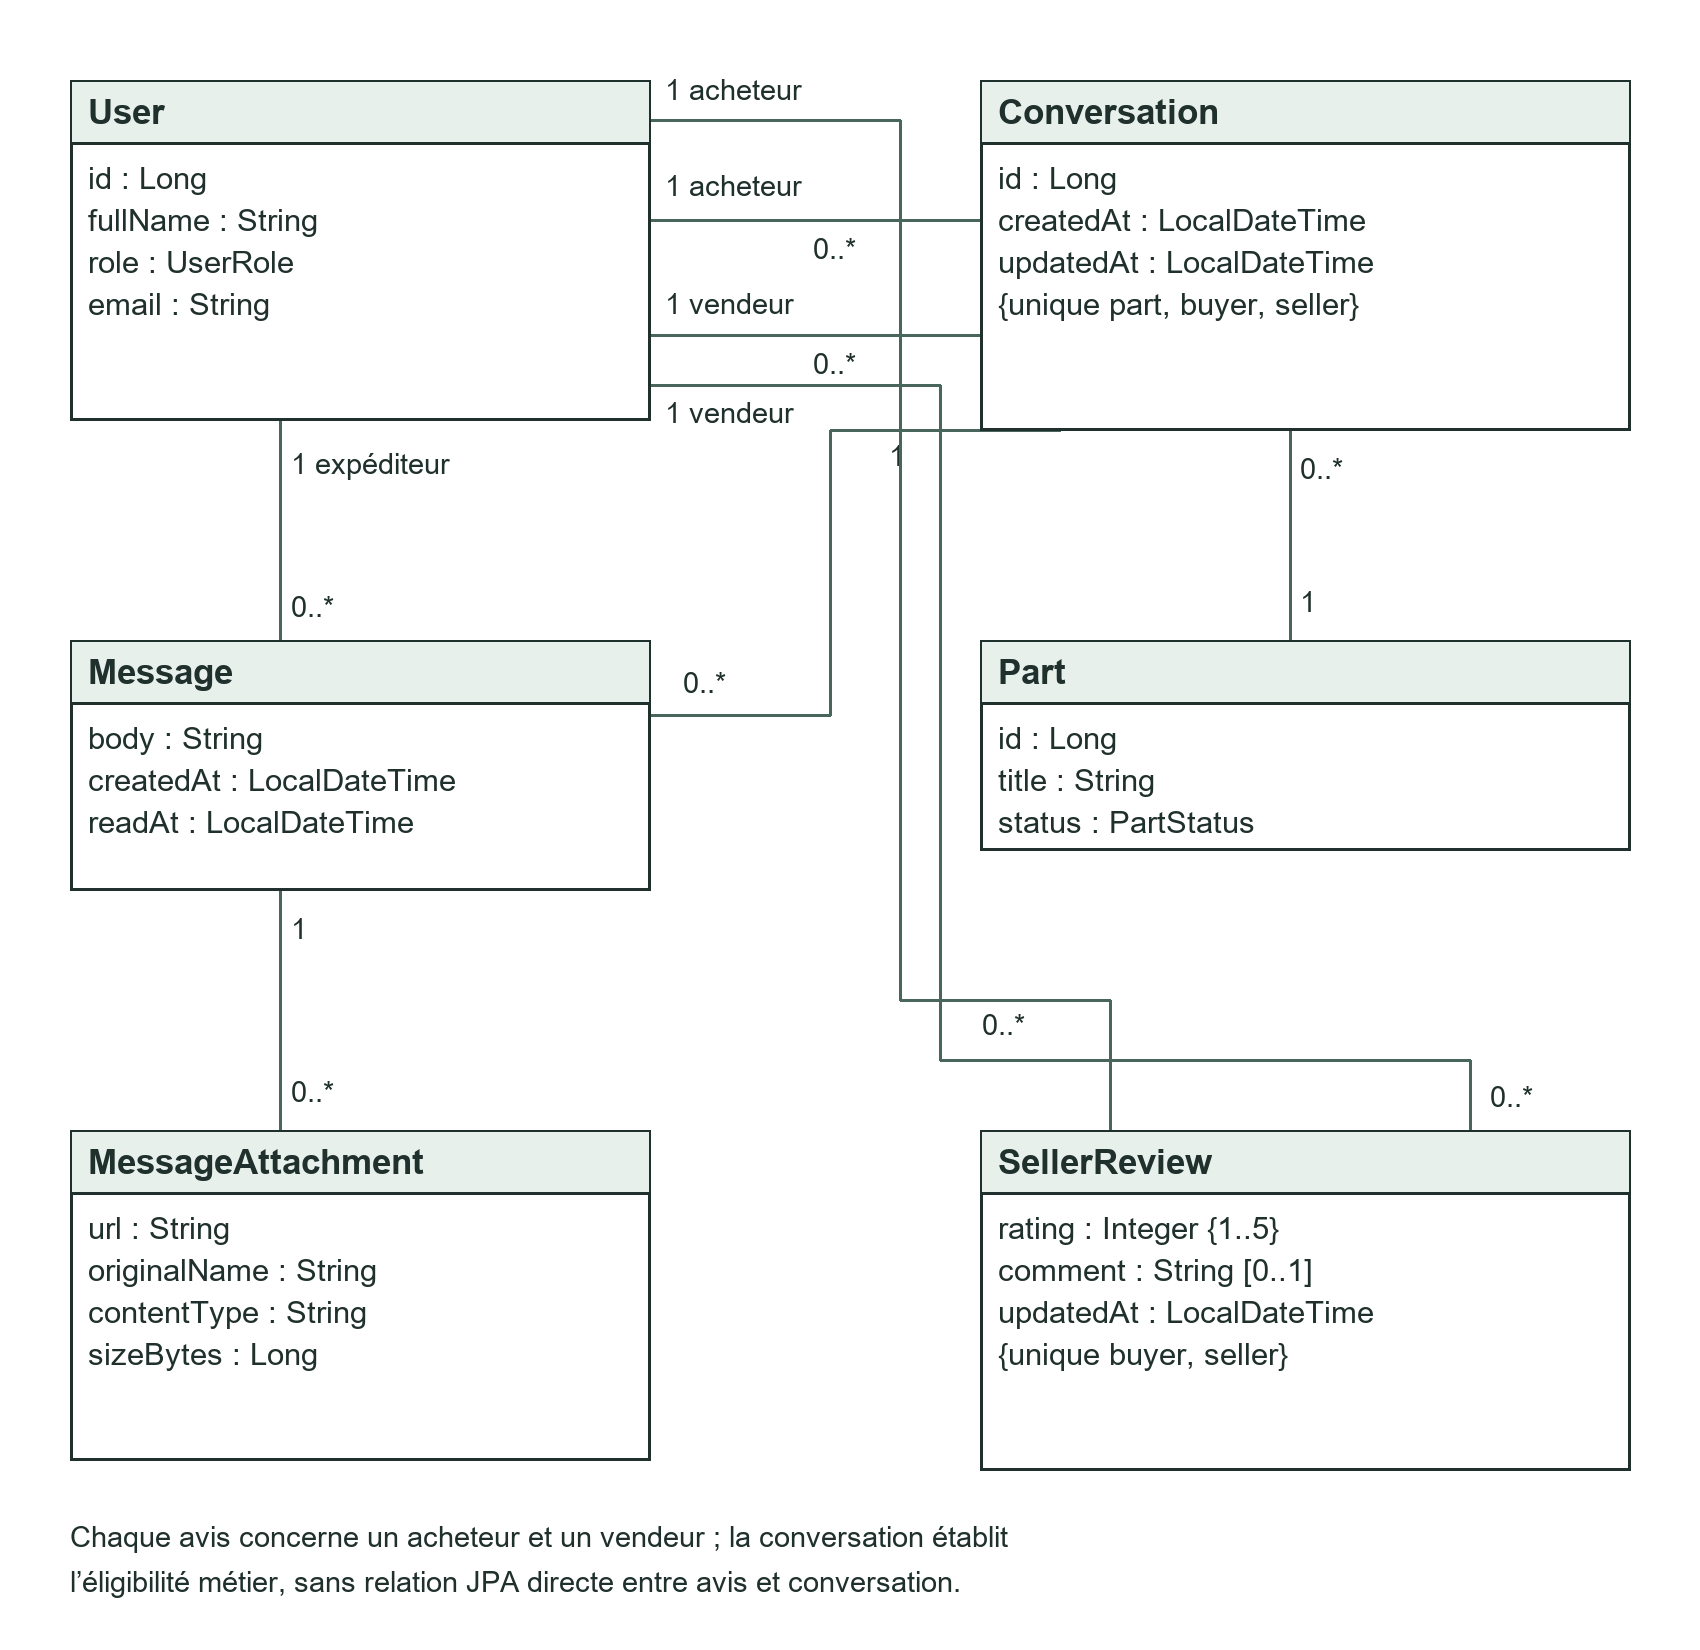
\includegraphics{images/figure-05.png}
\end{adjustbox}

\caption{Classes de communication et de réputation}
\label{fig:report-5}
\end{figure}

Une conversation relie exactement une annonce, un acheteur et un vendeur. Elle contient zéro à plusieurs messages ; chaque message a un seul expéditeur et zéro à plusieurs pièces jointes. Les avis référencent directement les deux utilisateurs. Les autorisations vérifient que l'expéditeur appartient à la conversation.


\clearpage

\subsection{Identité et personnalisation}

\begin{figure}[H]
\centering
\begin{adjustbox}{max width=\textwidth,max height=.64\textheight}
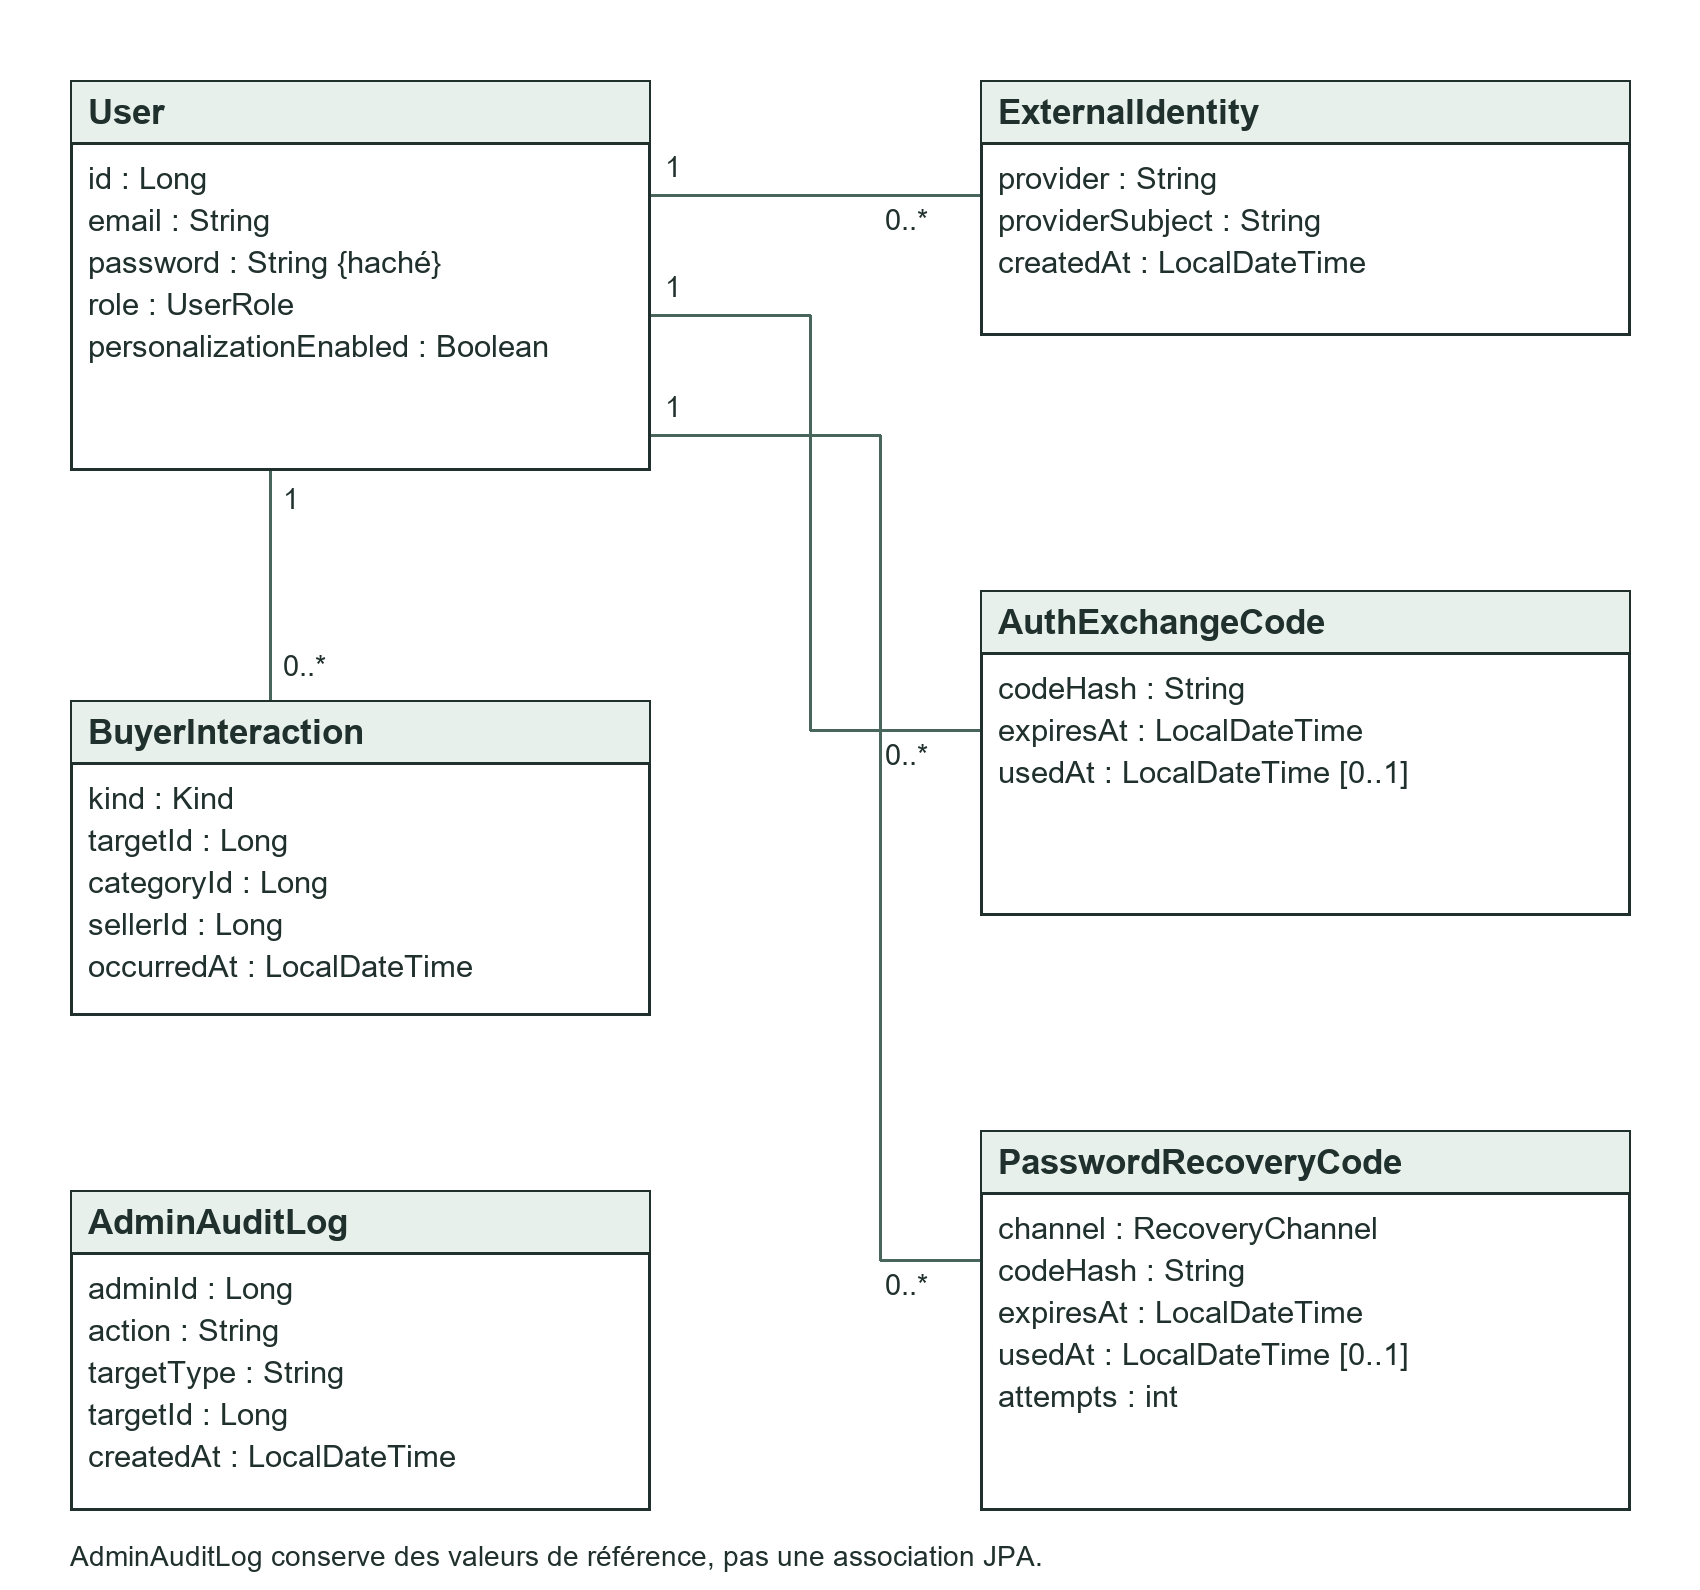
\includegraphics{images/figure-06.png}
\end{adjustbox}

\caption{Classes d'identité et de personnalisation}
\label{fig:report-6}
\end{figure}

Les codes temporaires sont associés à un utilisateur et stockés sous forme de condensat. BuyerInteraction contient des références numériques de contexte et n'établit pas de relations JPA vers Part ou Category. AdminAuditLog conserve un instantané d'identifiants et de libellés pour préserver la trace d'une action.


\clearpage

\subsection{Signalements et validation des vendeurs}

\begin{figure}[H]
\centering
\begin{adjustbox}{max width=\textwidth,max height=.64\textheight}
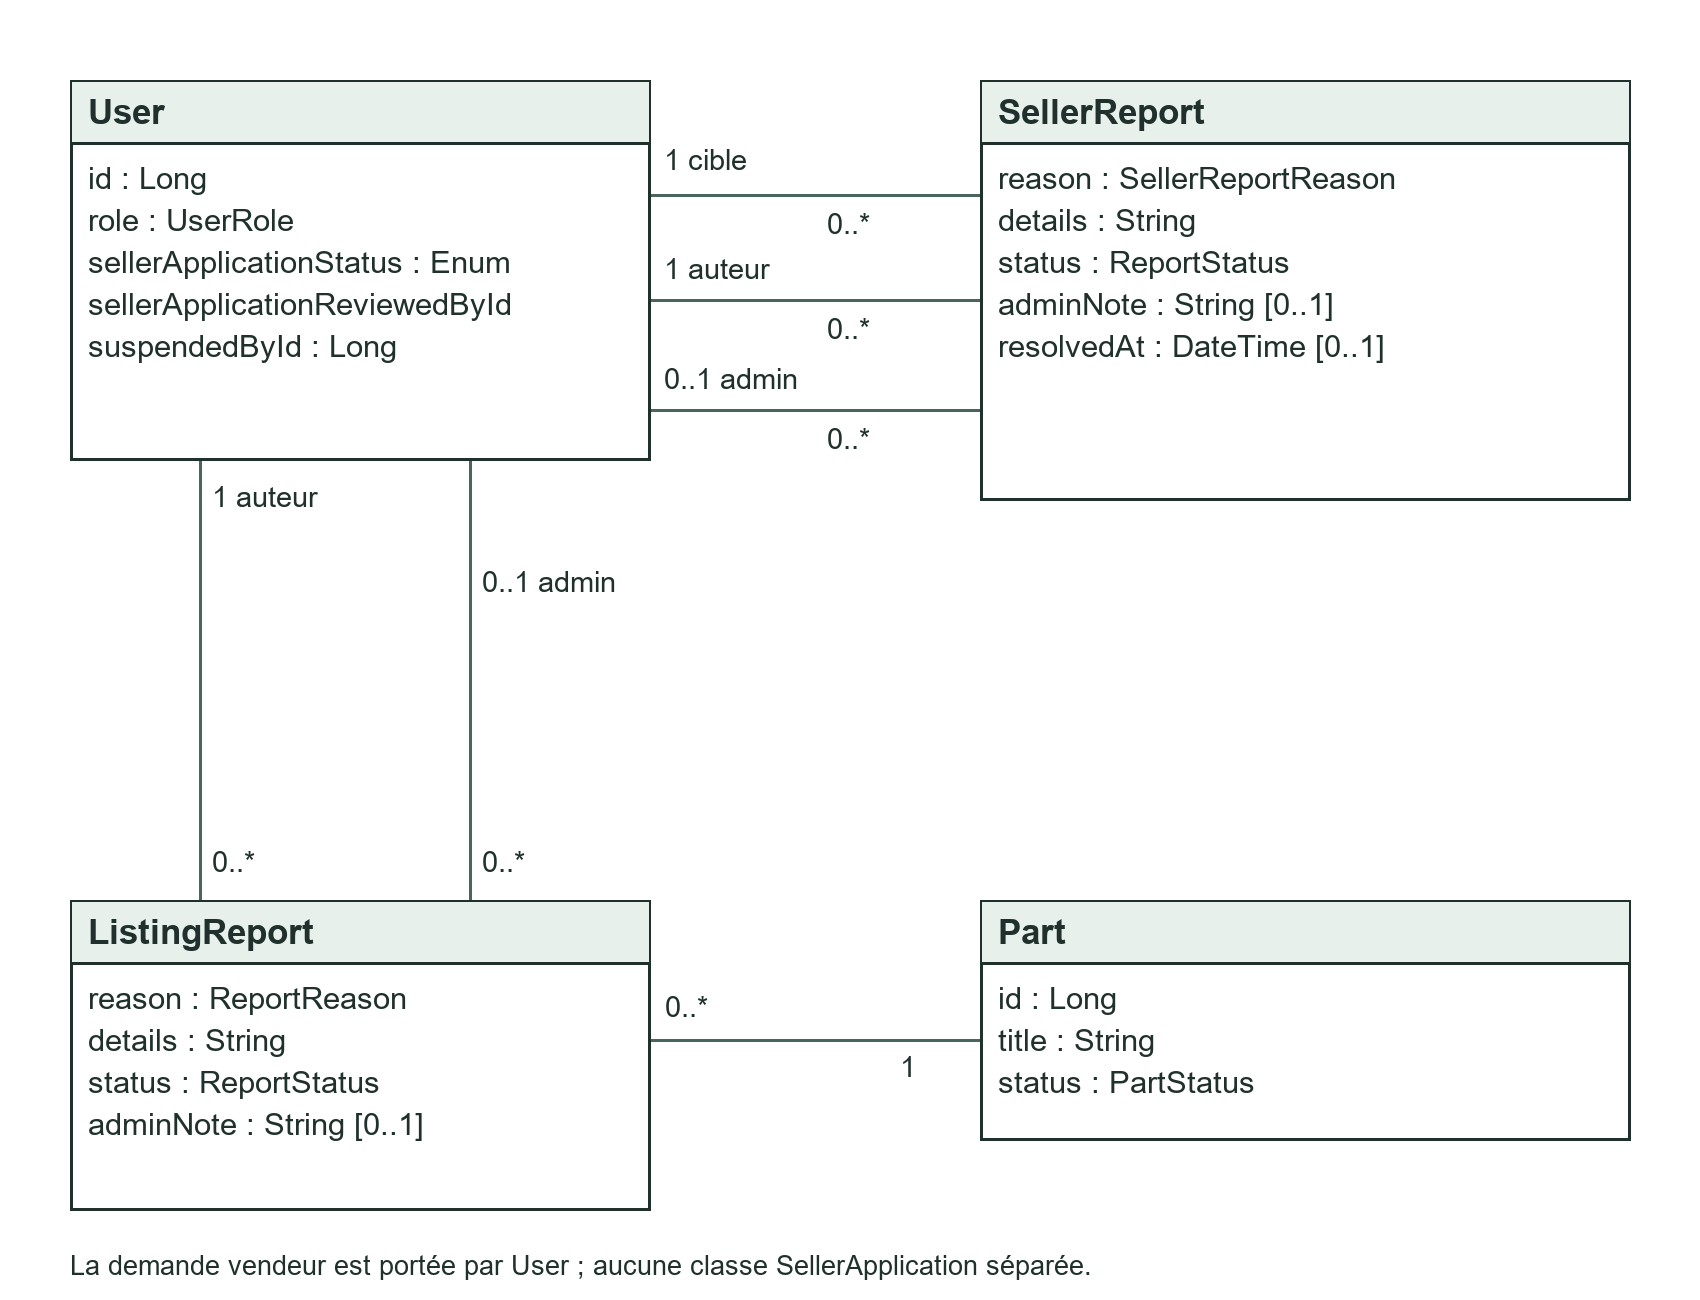
\includegraphics{images/figure-07.png}
\end{adjustbox}

\caption{Classes de modération}
\label{fig:report-7}
\end{figure}

SellerReport et ListingReport distinguent l'auteur, la cible et l'administrateur résolveur facultatif. La demande de passage vendeur est représentée par des champs de User, dont le statut et les dates de traitement. L'acceptation change le rôle ; le dépôt d'une demande ne crée pas automatiquement un vendeur.


Les structures de recherche, VIN, prix et vision sont des DTO ou des résultats temporaires de services. Elles ne créent pas de tables JPA supplémentaires. L'index Qdrant est reconstructible à partir de MySQL et n'est pas un second référentiel transactionnel. Les champs d'identité sont réservés aux DTO autorisés et ne sont pas tous exposés dans les profils publics.


\clearpage

\section{Conception de la recherche intelligente}

Une annonce active est transformée en document textuel normalisé contenant titre, description, catégorie, références et compatibilités. FastEmbed calcule son vecteur multilingue, stocké dans la collection Qdrant. Lors d'une requête, Qwen extrait un objet JSON. Le système fusionne cette sortie avec les contraintes lexicales et les filtres explicites, puis récupère des candidats sémantiques.


Le classement final applique un seuil minimal et vérifie les contraintes sur une même ligne de compatibilité. Les raisons visibles - par exemple « compatible Golf », « diesel », « position arrière » ou « système de freinage » - proviennent des champs réellement associés à l'annonce. La réponse est construite par Spring à partir des DTO actifs, ce qui empêche une prose générée ou un identifiant périmé de devenir une recommandation publique.


\begin{figure}[H]
\centering
\begin{adjustbox}{max width=\textwidth,max height=.64\textheight}
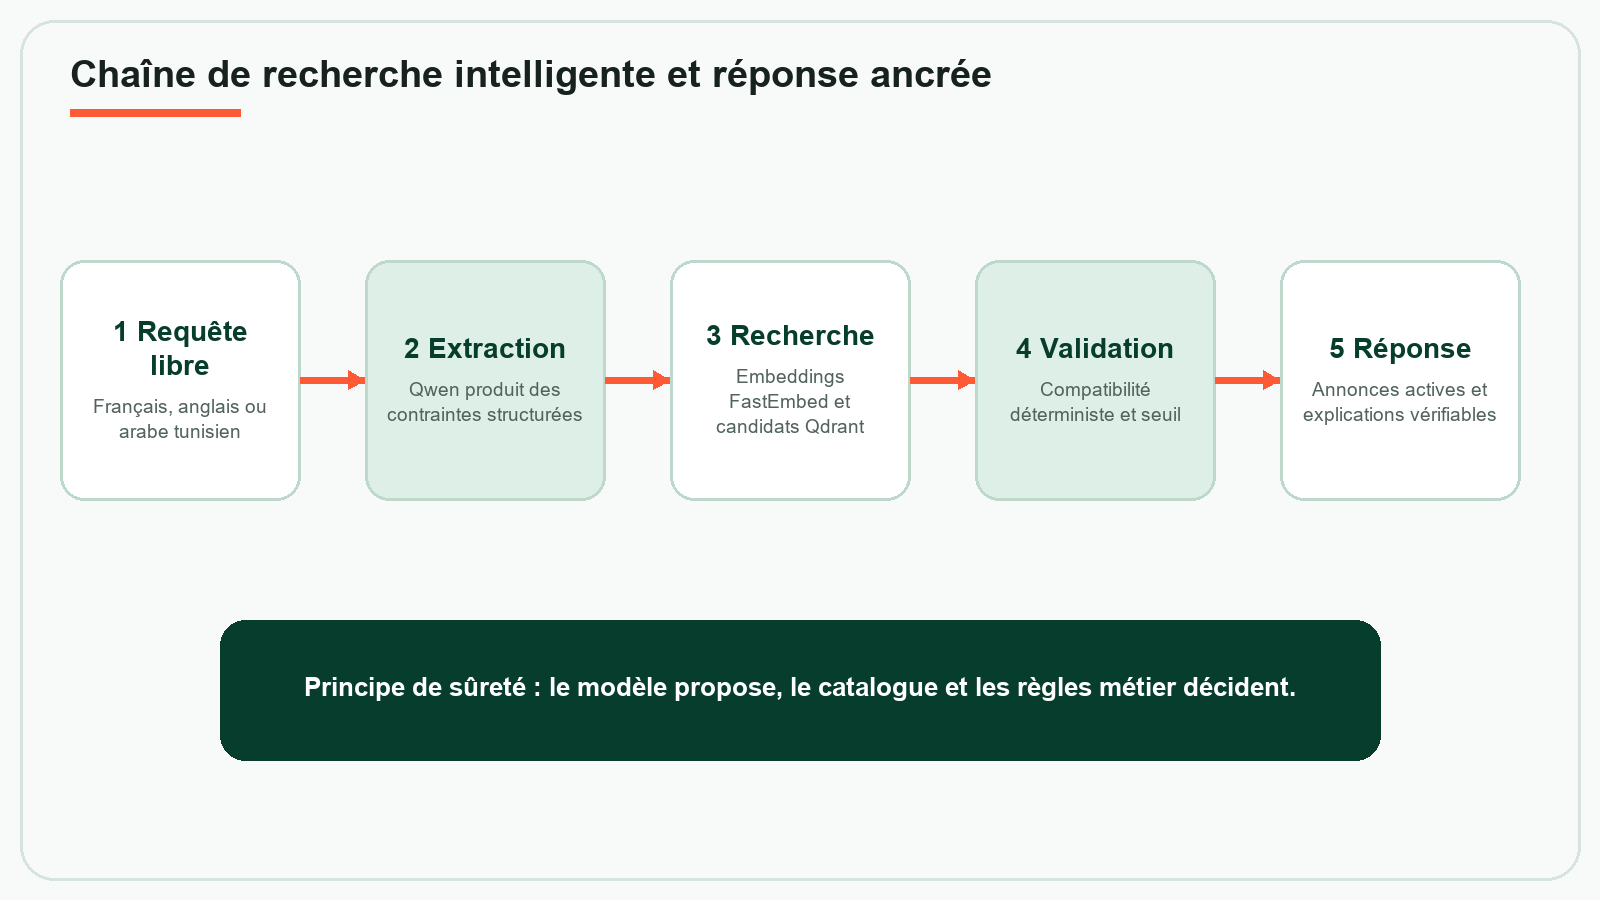
\includegraphics{images/figure-08.png}
\end{adjustbox}

\caption{Chaîne de recherche intelligente et réponse ancrée}
\label{fig:report-8}
\end{figure}

\section{Orchestration agentique finale}

La couche LangChain encapsule trois outils StructuredTool : search\_agent, compatibility\_agent et recommendation\_agent. Le routage est déterministe : la recherche s'exécute d'abord, la vérification des contraintes suit si nécessaire, puis les candidats personnalisés fournis par Spring peuvent être intégrés selon l'intention détectée. Il ne s'agit pas d'agents autonomes qui planifient librement des actions. Aucun outil ne crée, ne modifie ou ne supprime une donnée métier.


{\small\singlespacing\arrayrulecolor{tableline}
\begin{longtable}{|>{\raggedright\arraybackslash}p{\dimexpr 0.230\textwidth-2\tabcolsep-2\arrayrulewidth\relax}|>{\raggedright\arraybackslash}p{\dimexpr 0.250\textwidth-2\tabcolsep-2\arrayrulewidth\relax}|>{\raggedright\arraybackslash}p{\dimexpr 0.260\textwidth-2\tabcolsep-2\arrayrulewidth\relax}|>{\raggedright\arraybackslash}p{\dimexpr 0.260\textwidth-2\tabcolsep-2\arrayrulewidth\relax}|}
\hline
\rowcolor{tablehead} \color{white}\bfseries Agent & \color{white}\bfseries Entrées & \color{white}\bfseries Sortie autorisée & \color{white}\bfseries Garde-fou \\ \hline
\endfirsthead
\rowcolor{tablehead} \color{white}\bfseries Agent & \color{white}\bfseries Entrées & \color{white}\bfseries Sortie autorisée & \color{white}\bfseries Garde-fou \\ \hline
\endhead
\hline\endfoot
Recherche & Texte et filtres & Identifiants candidats & Limite et seuil de pertinence \\ \hline
\rowcolor{tablerow} Compatibilité & Contraintes et fiche annonce & Candidats conservés après revalidation & Règles catalogue prioritaires \\ \hline
Recommandation & Candidats assainis fournis par Spring et limite & Suggestions et raisons & Pas de données inter-utilisateurs \\ \hline
\rowcolor{tablerow} Orchestrateur & Intention utilisateur & Plan court et réponse structurée & Lecture seule, délai et nombre d'appels bornés \\ \hline
\end{longtable}
}


\section{Sécurité}

\begin{itemize}
\item identité extraite du contexte JWT, jamais d'un identifiant fourni librement par le client ;

\item autorisation par rôle au niveau des routes et réévaluation de la propriété dans les services ;

\item codes OAuth courts, à usage unique, sans JWT dans l'URL de redirection ;

\item codes de récupération expirables, nombre d'essais limité et réponses non révélatrices ;

\item jetons WebSocket courts et à usage unique pour éviter de transmettre le JWT dans une chaîne de requête ;

\item signature réelle des fichiers image contrôlée en plus du type MIME déclaré ;

\item jeton interne partagé entre Spring et FastAPI pour les opérations d'indexation ;

\item limitation de débit, concurrence bornée, cache court et délai maximum sur l'endpoint IA public ;

\item secrets chargés depuis l'environnement et exclus de Git.
\end{itemize}

\clearpage

\section{Conception de la messagerie}

La messagerie suit un modèle conversationnel unique par contexte d'annonce. Le chargement initial place la vue sur le dernier message, tandis que le contenu reste dans une zone de hauteur limitée et défilable. Les événements WebSocket mettent à jour l'interface sans recharger la page. Les images jointes sont stockées via le même contrat que les images d'annonces, avec des limites dédiées.


\begin{figure}[H]
\centering
\begin{adjustbox}{max width=\textwidth,max height=.64\textheight}
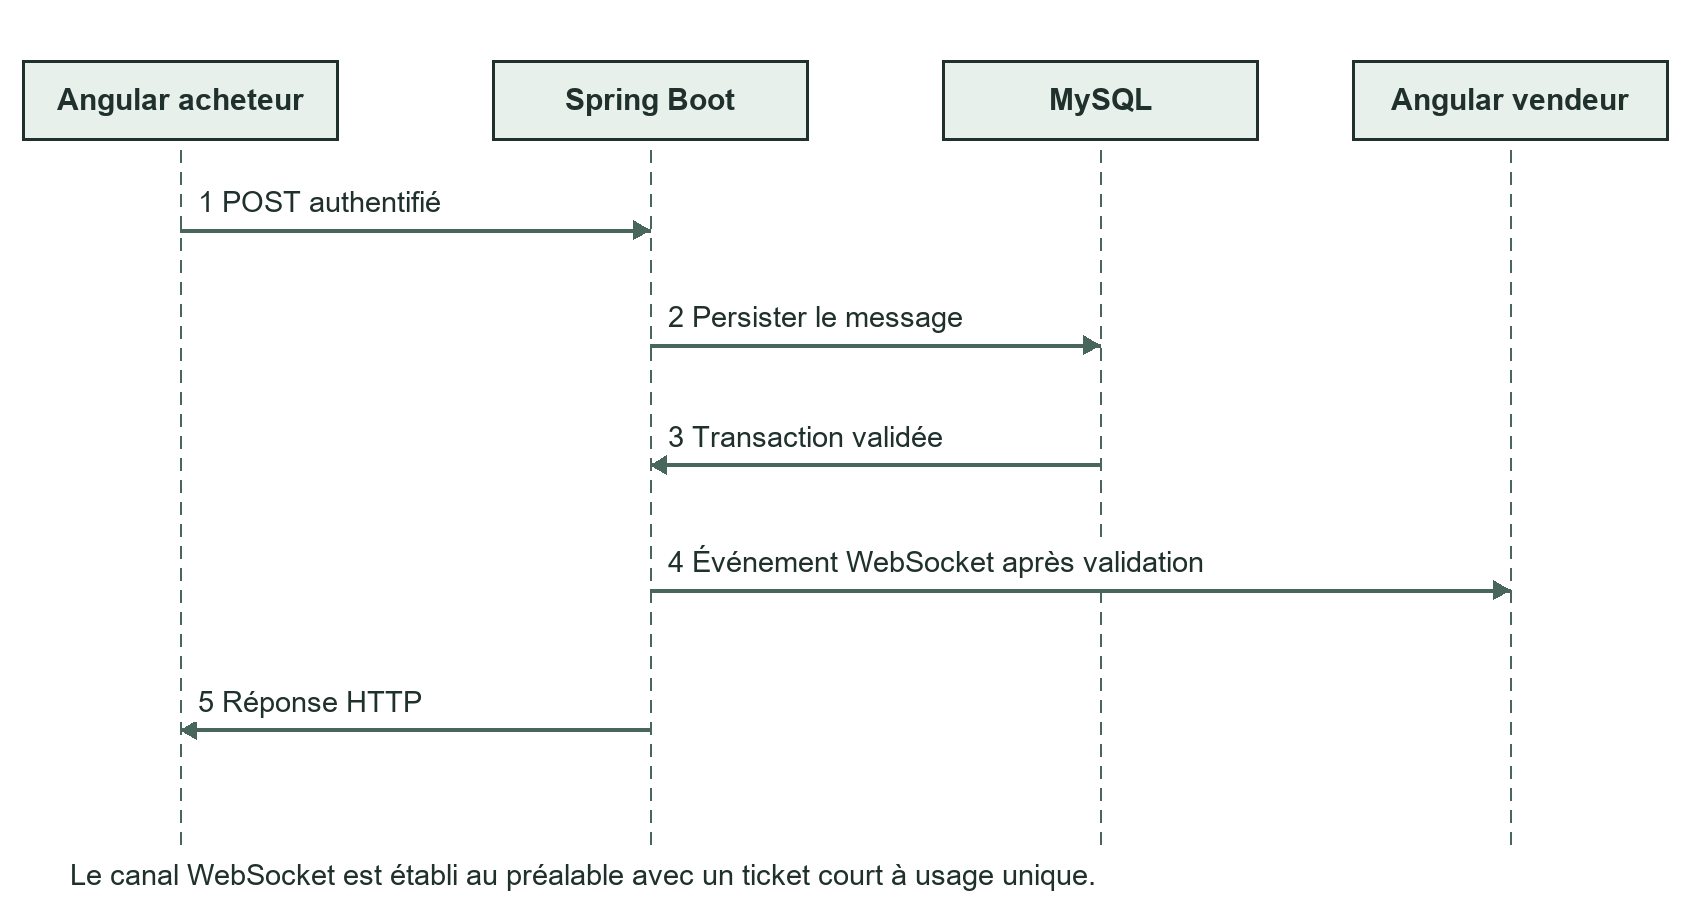
\includegraphics{images/figure-09.png}
\end{adjustbox}

\caption{Séquence simplifiée de la messagerie instantanée}
\label{fig:report-9}
\end{figure}

\clearpage

\section{Conception de la recommandation}

Le moteur combine compatibilité déclarée, catégories sauvegardées, vendeurs contactés, popularité et récence. Les préférences véhicule agissent comme contrainte forte. Les interactions comportementales sont dédupliquées, limitées à 200 enregistrements, pondérées avec une demi-vie de trente jours et ignorées après quatre-vingt-dix jours. Le score reste un rang interne et n'est jamais présenté comme un pourcentage de compatibilité.


\begin{figure}[H]
\centering
\begin{adjustbox}{max width=\textwidth,max height=.64\textheight}
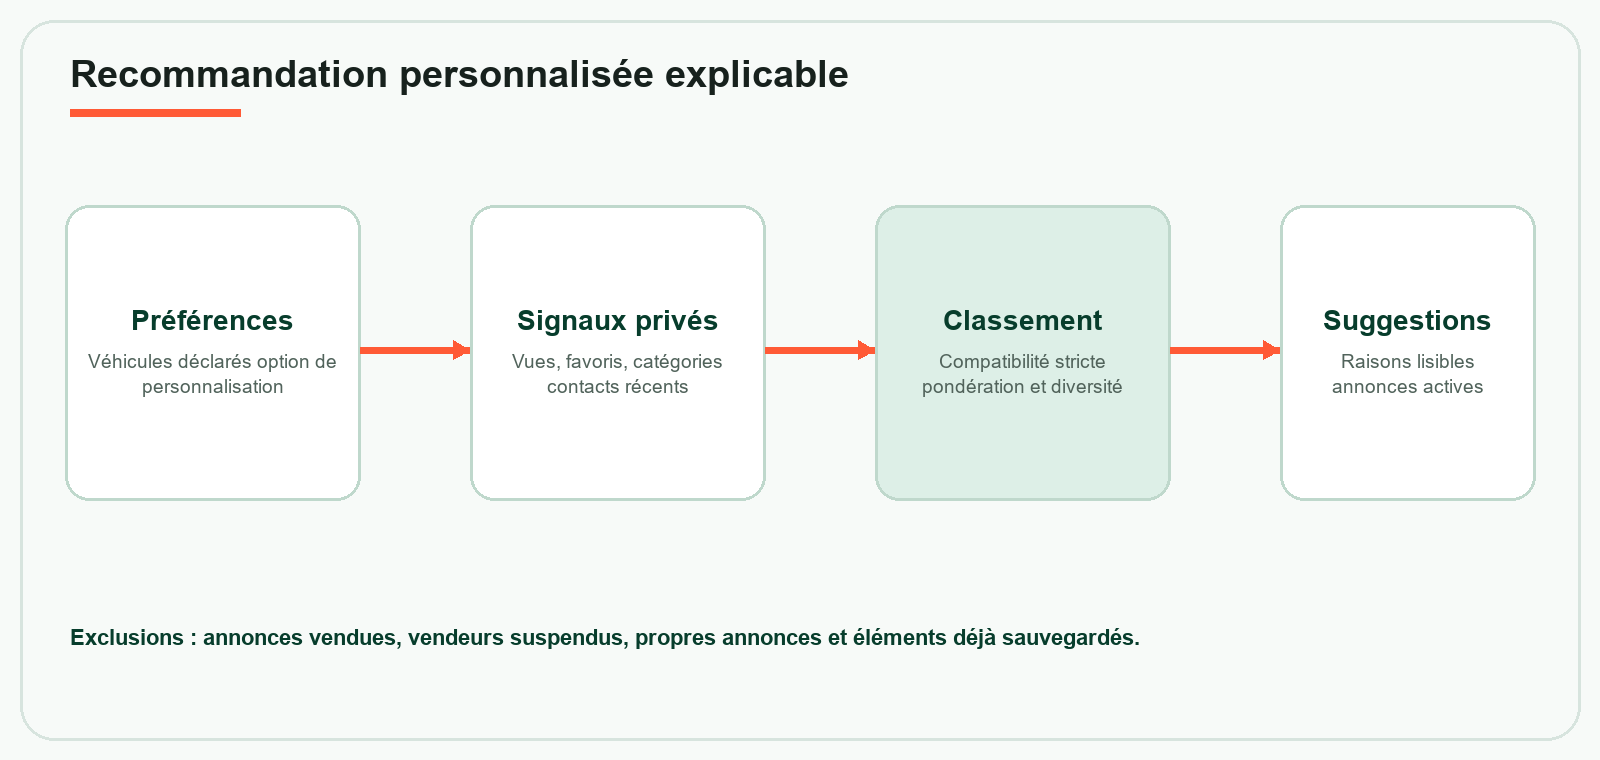
\includegraphics{images/figure-10.png}
\end{adjustbox}

\caption{Recommandation personnalisée explicable}
\label{fig:report-10}
\end{figure}
